

\documentclass[sigconf]{acmart}

%% \BibTeX command to typeset BibTeX logo in the docs
% \AtBeginDocument{%
%   \providecommand\BibTeX{{%
%     \normalfont B\kern-0.5em{\scshape i\kern-0.25em b}\kern-0.8em\TeX}}}

%% Rights management information.  This information is sent to you
%% when you complete the rights form.  These commands have SAMPLE
%% values in them; it is your responsibility as an author to replace
%% the commands and values with those provided to you when you
%% complete the rights form.
\setcopyright{acmcopyright}
\copyrightyear{2018}
\acmYear{2018}
\acmDOI{10.1145/1122445.1122456}

%% These commands are for a PROCEEDINGS abstract or paper.
% \acmConference[Woodstock '18]{Woodstock '18: ACM Symposium on Neural
%   Gaze Detection}{June 03--05, 2018}{Woodstock, NY}
% \acmBooktitle{Woodstock '18: ACM Symposium on Neural Gaze Detection,
%   June 03--05, 2018, Woodstock, NY}
% \acmPrice{15.00}
% \acmISBN{978-1-4503-XXXX-X/18/06}

\usepackage{array}
\usepackage{tabularx}

%% end of the preamble, start of the body of the document source.
\begin{document}

%% Title used for page headers
\title{Taxulator – The Smart Way to File Taxes}
\pagestyle{plain}
% \rfoot{Page \thepage \hspace{1pt} of \pageref{LastPage}}

% Authors
\author{Elisha Coad}
\affiliation{%
  \institution{Department of Computer Science}
  \institution{University of Idaho}
  \city{Moscow}
  \country{USA}}
\email{coad1223@vandals.uidaho.edu}

\author{Cade Disselkoen}
\affiliation{%
  \institution{Department of Computer Science}
  \institution{University of Idaho}
  \city{Moscow}
  \country{USA}}
\email{diss7248@vandals.uidaho.edu}

\author{Ryan Rapier}
\affiliation{%
  \institution{Department of Computer Science}
  \institution{University of Idaho}
  \city{Moscow}
  \country{USA}}
\email{rapi3147@vandals.uidaho.edu}

\author{Hasan Jamil}
\affiliation{%
  \institution{Department of Computer Science}
  \institution{University of Idaho}
  \city{Moscow}
  \country{USA}}
\email{jamil@uidaho.edu}


%% Abstract
\begin{abstract}
  For decades, taxes have remained the same. People are expected to keep meticulous record of all their income and spending over the year and then spend hours filling out a tax report. While the effort put into this is commendable, what if there’s a better way? In this paper, we describe the implementation of Taxulator \cite{TaxulatorDemo}, a quicker and easier way to file yearly taxes. Through collecting forms from the appropriate parties beforehand, the individual taxpayer is able to file taxes in a matter of minutes.
\end{abstract}

% CCS Concepts
\ccsdesc[500]{Information systems~Data management design and models}
\ccsdesc[500]{Computing methodologies~Information extraction}
\ccsdesc{Computing methodologies~PDF parsing}

% Keywords
\keywords{tax reports, query language, congregate user system, information extraction, user profile management system}

%% This command builds the first part of the formatted document.
\maketitle

\section{Introduction}
\subsection{Motivation}
In the United States of America, taxes have always been a complex system. It requires much leg work on the individual taxpayer and because of this the process is often dreaded. This is the motivation behind the Taxulator program, to streamline the tax filing process. Our aim is to make so that once the appropriate information is in place, a user can submit their tax report with the click of a button.

An additional motivation for Taxulator is to bring the myriad of benefits of technology to tax filing. Such benefits include security, clarity, and easy record keeping. By receiving private financial information directly from the source, without the possibility of interception, we provide security. By providing additional information throughout the tax filing process, so that fewer mistakes are made overall, we provide clarity. And we also bring better record keeping, for a digital report is much easier to find and pull up than searching through boxes of old files.

\subsection{Research}
Previous research shows there are already a few tax solutions on the market. One can hire a professional tax accountant to do their taxes for them, however this method requires handing off private information and can be a bit costly. There also are also several tax websites which aim to make tax filing an easier process, such as TurboTax and FreeTaxUSA. However, there are very few that use a centralized user filing scheme, meaning that most websites still require the individual taxpayer to upload all of their employer forms, investment interest forms, rental income forms, and the list goes on. What we propose is that these forms are submitted directly by their respective parties, helping reduce the overall amount of confusion and drudgery for the everyday user.

\subsection{Challenges}
As one might expect, a collaborative tax filing process such as the one Taxulator is looking to employ has its challenges. For one, it’s a scheme that requires the cooperation of multiple parties to work. For a single tax filing, employers must report salaries, banks must report investment interests, rentals must be reported by the renters and so on. To help speed up its adoption rate, Taxulator would be deployed in controlled areas where the companies and banks in that area are encouraged to adopt Taxulator as part of their process for the yearly tax season. If we can get a few cities fully on-board with the Taxulator system, the hope is that its usefulness will catch on and it will spread outward to other cities.

Another challenge with creating any digital system that deals with finances is security. We will be dealing with highly private information and as such will need highly secure systems. To do this, our goal is to limit our access to the customer’s info and documents as much as possible, so that only the parties who need the information will have access. We will also be utilizing top-of-the-line encryption methods so that in the unlikely event there is a security breach, all data will be unrecognizable.

The last challenge that will be discussed is the difficulty of collating data from multiple different sources and documents into one place. There will be multiple forms from multiple enterprises, each requiring different treatment. Not only will the documents need to be scrapped, each type of document will require a custom way to scrap the data. This challenge though can be overcome through simply brute force. We will ensure we have methods of handling each unique form. In the odd case of a form being needed that we don’t have, we will give the user an option to flag the case so that we can add the case for future users.

\section{Design and Architecture}
Taxulator will need to collect data from both the individual taxpayer as well as from organizations. Because of this, our website implements two ways to use the website, as an individual and as an organization. The individual’s side of the website will give options to file a new tax return, resubmit a tax return, and to review previous filings. The organization side of the website will allow organizations to manage an employee/customer database and to submit forms for specific employees/customers. Both will be assigned a unique 20-digit identifier upon registration.

When a user lands on the site, they will be asked to create an account. This will set up some of the basic information for the user that can be used for the tax filing process and this is also when a unique 20-digit identifier will be assigned. When the user goes to file their taxes, Taxulator will automatically link all appropriate forms (provided by other organizations) to the taxpayer’s session. The user can verify that all the right forms were included before carrying on. If anything is missing, the user will have to option to upload the form manually. The user will also have the option to report their own expenses.

\begin{figure}[H]
  \label{UserFlow}
  \centering
  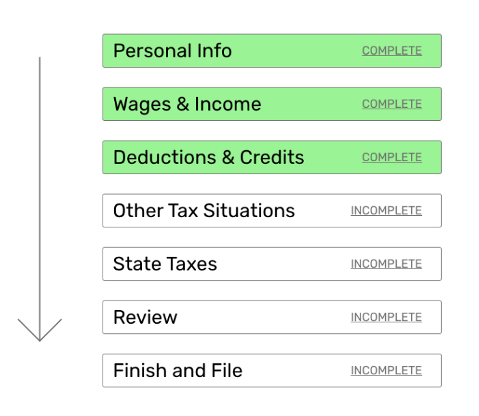
\includegraphics[width=\linewidth]{Images/UserFlow.png}
  \caption{Tax Report Session Flow}
\end{figure}

The next step is to calculate the users adjusted taxable income. To do this, the user will check off which deductions they are eligible for. Then student loans, home mortgage interests, job-related expenses, etc. will be taken into effect producing the user’s adjusted taxable income. The adjusted taxable income is then taxed using a graduated scale, and the user is notified of which percentage rate will be applied.

\begin{figure}[H]
  \centering
  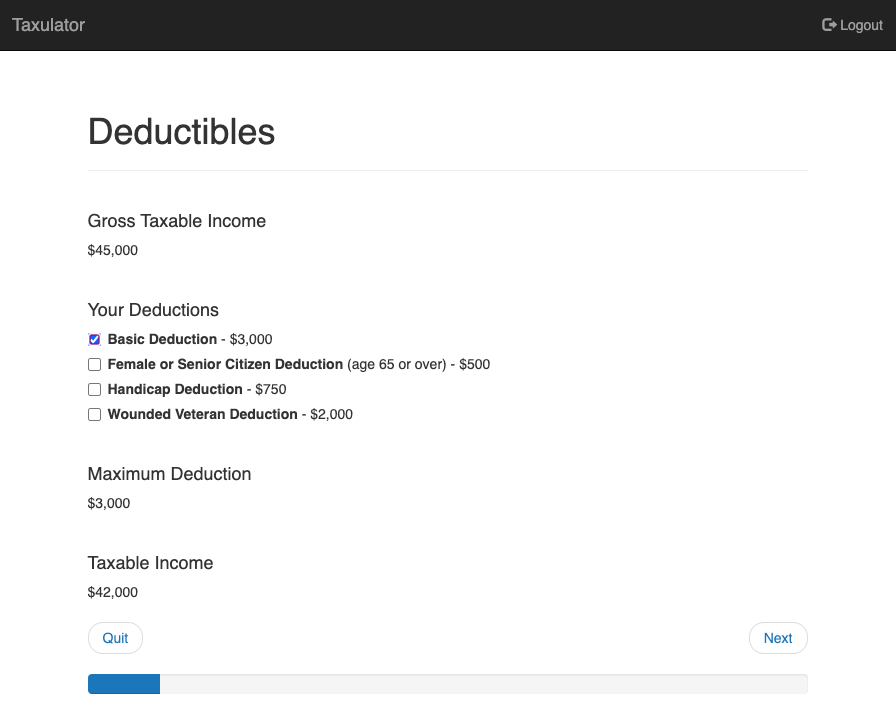
\includegraphics[width=\linewidth]{Images/Form2.png}
  \caption{Tax Payer Deductibles Form}
  \label{TaxableIncome}
\end{figure}

Then the minimum annual city tax is ensured using a database of the city tax minimums in the USA. After this, the user reports their employers, businesses or farms owned, and any houses they own. The user also must report home rentals. The first time any of these are entered they will get added to a database for future use. Once added to the database, the user will be able to select them from a drop-down list.

Lastly, Taxulator will prepare the tax return. It will attach all necessary documents, cross reference incomes and deductions, and verify all reports. Taxulator also will show the taxpayer if they are due for a return and if so of how much. At this point the user can sign and submit the report.
If the user wishes to modify the report, they can create a copy of it and then resubmit a new report. All submitted reports are retained and viewable from the dashboard of the website.

\subsection{Database Scheme}
Taxulator uses a session-centric database scheme. What this means is that as a user files a tax report, all correlated information will be stored in a session. Upon submission, this session will be added to the session database for future reference and retrieval. Refer to Figure \ref{DBSchema} for the database scheme we decided to use.

\begin{figure}[H]
  \centering
  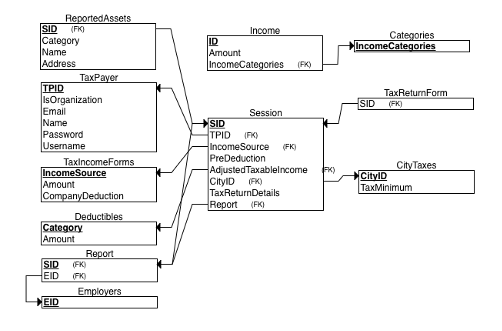
\includegraphics[width=\linewidth]{Images/DBSchema.png}
  \caption{Session Database Scheme}
  \label{DBSchema}
\end{figure}

We used this scheme because it allows for each category to be compartmentalized, and then retrieved when needed for the session. Since the user will be filing a new tax report every year, every report can just be saved as a session. Now something important to note is that as a user is going through submitting their tax return, all of that session's information will be stored client-side. This achieves multiple ends. First and foremost, if the user decides to quite filing midway, we wanted a way to store the data without entering an incomplete entry into our database. Storing it client-side allows that session to be temporarily suspended until the user decides to continue where they left off or discarded. Upon completion of filing taxes, the client-side session will be submitted as an entry to the database. This minimizes the need to place unstable data within our database.

\begin{table}[H]
\begin{center}
  \caption{Tax Payer Table Example}
\begin{tabularx}{0.45\textwidth} { | m{1cm} | m{.8cm} | m{1cm} | m{1cm} | m{1cm} | m{1cm} | }
%  \hline
%  \multicolumn{6}{|c|}{Tax Payer Table} \\
 \hline
 PID & IsOrg... & Name & Email & Username & Password \\
 \hline
 \hline
 232134... & 1 & Payton Mann & yledne... & wilder... & 43d3!S...\\
 \hline
 412312... & 0 & Juston Schuppe & kutchm... & emardr... & d1560a...\\
 \hline
 122134... & 0 & Pat Hood & vstant... & kasand... & 66cf0a...\\
 \hline
 774103... & 1 & Dwight Adams & lauren... & eeichm... & d51347...\\
 \hline
\end{tabularx}
\end{center}
\end{table}

\subsection{Stack}
Our stack implements two core layers, the client and the server. The client can be broken down further into the frontend and the backend. The server manages our database.

On the client side, we used HTML, CSS, and JavaScript to handle the frontend. We also implemented the CSS framework Bootstrap to handle much of the styling. We used PHP on the backend to interface with our MySQL database system.

On the server side, Apache was used for hosting our web server. Using Apache paired with the MySQL database on phpMyAdmin, we were able to get a fairly functional interface between the client and the server.

\begin{figure}[H]
  \label{Stack}
  \centering
  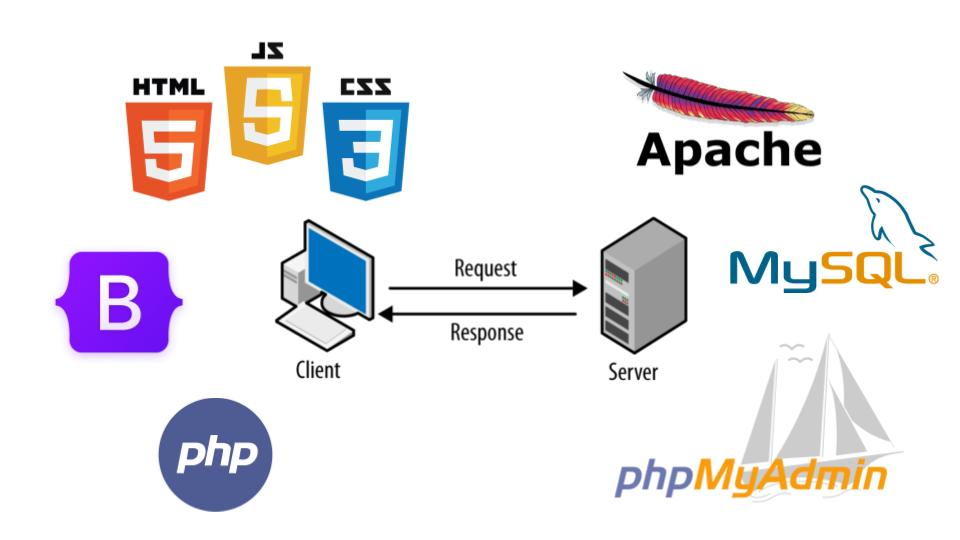
\includegraphics[width=\linewidth]{Images/ClientServer.jpg}
  \caption{The Client Server Stack}
\end{figure}

To help us get familiar working with such a stack, we created a sandbox page \cite{Sandbox}, based off of Joel’s code. We used this for testing out queries with the data. The sandbox allows for selecting a database to work with, typing in a query, and then submitting and getting the output. This was useful during the development stage of our site as it allowed for quick testing of queries to ensure they worked. This also helped us get a better understanding of how to work with multiple layers of the stack. By using PHP as the middle man, we were able to send queries to our database and then output the results.

\subsection{Functionality}
Taxulator’s core functionality is to allow users to file taxes quickly and easily. Several features come together to achieve this. Here are Taxulator’s primary features:
\begin{itemize}
\item Landing Page
\item User Profile System
\item User Dashboard
\item Business Dashboard
\item Data Forms
\item Records of Previous Sessions
\item Database of Tax-related Information
\end{itemize}

\subsection{Challenges}
While working on Taxulator, we came across many challenges. These included data generation, connecting to the server, and learning how to work with PHP. Many of the team hadn't had any experience with web programming, so we conducted much research on the subject to help us get started. While the challenges we faced did slow down our development, they also helped us learn how to overcome difficulties and how to be adaptable.

\paragraph{Data generation}
During the early stages of the project, one of the pressing issues was how we could fill the database with dummy data to test with. After hearing in class that dummy data could be generated with a python package named \textit{Faker}, we began our research. After a couple weeks of research and little progress, it was decided to discard the python package and find a dummy data generator. We tested a few more different generators and settled on one called \textit{FillDB} \cite{FillDB}. The challenge with data generation mainly came from having to spend many hours researching the python program and trying to get it to work. Ultimately, the decision to redirect our course was more beneficial, as it would have likely taken a considerable amount of more time to try and get \textit{Faker} working. After switching to the online data generator \textit{FillDB}, we were able to generate the data within only a couple hours and fill our database with dummy data.

\paragraph{Connecting to the server}
Later in the project, after setting up the database scheme and filling it with dummy data, our next task was to write PHP and HTML code to connect our database to the user interface. We downloaded FileZilla and attempted to login but got an error that said credentials were incorrect. After attempting to login on multiple different FTP programs and reentering the credentials, we were still rejected. We emailed the professor and subsequently the TA, though communication was slow. Unfortunately, while we tried to get as much as we could done during the meantime, all of our work having to do with the PHP code was practically on hold because we needed access to the server in order to set things up correctly. This slowed down our work considerably, but we tried to do what we could. Finally, a couple of weeks and emails later, we retested the credentials and were able to gain access. We are still unsure as to the reason for what was causing the error, but were thankful it got figured out.

\paragraph{Lack of sufficient knowledge in PHP}
Our last task was to connect the backend to the frontend through PHP code. None of the team members had had previous knowledge of PHP, so there was a steep learning curve we all went through. We spent many hours with PHP to try to get a sandbox up and running. This unfortunately ended up taking longer than expected, which made it so that we did not have time to implement many of the features we originally planned on completing. However this sandbox \cite{Sandbox} was extremely helpful for us to get a grasp of PHP and also helped us write queries for the Taxulator site.

\subsection{Design Choices}
Filing taxes is a complicated system. That's why we wanted Taxulator to be as intuitive as possible. When landing on the Taxulator homepage, the user will have the option to sign up or log in. Right underneath these options will also be a prompt for businesses. That will lead to a similar homepage, but with a sign up and log in for businesses. We chose this design because we realize the bulk of our users will be individual tax payers, so we want it to be quick and easy for them to know what to do. If a business happens upon the website though, we want them to find their portal. Alternatively we also will provide a \textit{taxulator.com/business} url for business to go directly to their side of the website.

\begin{figure}[H]
 \label{Home}
  \centering
  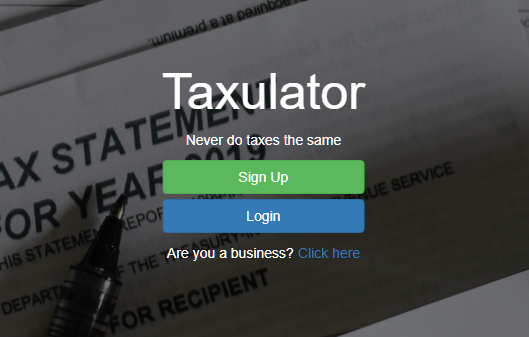
\includegraphics[width=\linewidth]{Images/TaxulatorHome2.png}
  \caption{Taxulator Landing Page}
\end{figure}

Once logged in, the user will be taken to their dashboard. This is their personal home page. From here they can start a new tax report or view previous reports. They can also download previous reports in the form of a PDF if needed. We chose a dashboard design because we needed a place that the user can feel grounded to as they go about filing taxes.

\begin{figure}[H]
  \label{Dashboard}
  \centering
  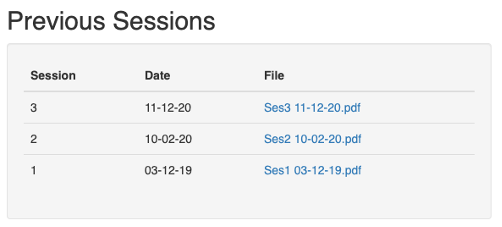
\includegraphics[width=\linewidth]{Images/Dashboard.png}
  \caption{Dashboard View of User’s Previous Sessions}
\end{figure}

For the design language, we decided to go with a clean and minimal style. We used an open-source CSS framework called Bootstrap \cite{Bootstrap} to quickly and efficiently get our designs up and running. Using Bootstrap helped us stay consistent in much of our styling. However, we did still use some CSS for spacing and such where needed.

\subsection{Platform Selection}
When we first started Taxulator, we conducted much research to decide which platforms we were going to be using. With so many options, it was hard to narrow down the best ones. However, we made some choices, so here are the main platforms we decided to go with.

\paragraph{ERDPlus}
We used a software tool called ERDPlus to generate our Relational Schema diagrams. It’s a free tool online which allows for easy database modeling using a cloud-based system. ERDPlus also allowed us to brainstorm out what our primary keys were going to be and how we wanted to structure our database \cite{ERDPlus}.

\paragraph{FillDB}
FillDB allowed us to be able to quickly generate a large volume of data in MySQL format in order to populate our database. Most of our data was generated this way, entries such as taxpayers, employers, city tax rates, etc \cite{FillDB}.

\paragraph{Trello}
To keep track of who was working on what, and what still needed to get done, we used a team management tool called Trello. Trello made it easy to see who was working on what and also to see what we still had left to get done. We could tag the importance of each task as well as link to useful resources for future reference. This tool helped streamline the development process and provided clarity when there was a plethora of moving parts \cite{Trello}.

\begin{figure}[H]
  \label{Trello}
  \centering
  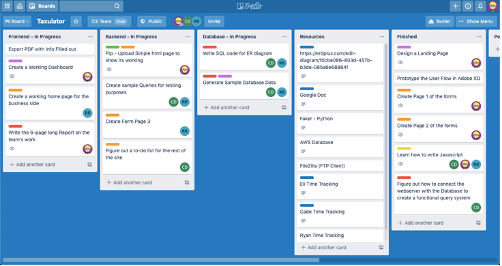
\includegraphics[width=\linewidth]{Images/TrelloBoard.png}
  \caption{Snapshot of Our Team’s Trello Page}
\end{figure}

\paragraph{Adobe XD}
Adobe XD is a powerful prototyping tool that we used to get an idea of where we were going. View Figure \ref{Prototype} to see the screens made. The blue arrows show the flow of the screens. This allowed us to step through the pages in a prototype before we even got to programming, so we could have a clear picture of where we were headed \cite{AdobeXD}.

\begin{figure}[H]
  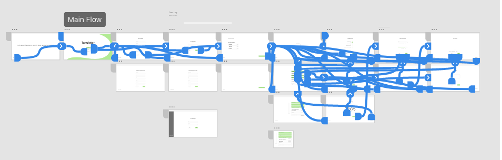
\includegraphics[width=\linewidth]{Images/Prototype.png}
  \caption{Adobe XD Taxulator Prototype}
  \centering
  \label{Prototype}
\end{figure}

\paragraph{GitHub}
We tried to use the version control software GitHub to track changes made to the code base. Unfortunately, we did not get to implement its use as much as we would have liked, but nonetheless it is still a valuable tool. We added our final code to GitHub for sharing \cite{TaxulatorCode}. If we were to carry this project further, we would like to transition to a purely GitHub workflow to keep track of changes made and to have backups of our code base \cite{GitHub}.

\paragraph{phpMyAdmin}
phpMyAdmin is an online software tool we used to handle the administration over our MySQL database. After generating sample data with FillDB, we imported this data into phpMyAdmin to use with our website \cite{phpMyAdmin}.

\paragraph{Other Tools}
We also used other tools such as Adobe Illustrator \cite{Illustrator} and Adobe InDesign \cite{InDesign} to draft up user flows and for making presentations. Along the way, we also used Google Docs \cite{GDocs} for shared notes, MySQL Workbench \cite{Workbench} for testing queries, and Visual Studio Code \cite{VSCode} as our editor.

\section{Conclusion}
Taxulator has come a long way. That being said, there’s still a lot of work ahead of us to make a final product. There are many limitations to our current design, and many improvements that are in order.

\subsection{Current Limitations}
Currently there are many features that need to be refined in the project. Specifically, connecting the backend to the frontend has been a challenge and has still not been fully implemented. It has been a struggle to work through the different errors that came with PHP, so the software is currently limited by our ability with PHP.

\subsection{Future Improvements}
In order to improve, the first thing we would do is implement more backend to frontend PHP code. We would build out the forms and make sure they are working with the database. We could then work on a PDF generator to output a final PDF tax report when the user finishes their session. Additionally, we could refine the overall interface of the website, ensuring a consistent design language.

Other improvements would include executing a more comprehensive business side to the site. While with a limited time frame we had to prioritize the user side of the site, we recognize that the business side is also an integral part and would like to have built that out more. Also one other large part of the site that we weren't able to get to was the security side of the site. Finances require a high level of security, so we would have liked to spent a fair amount of time on securing users' information in the form of end-to-end data encryption.

We also wanted to add more complementary material to the tax filing process in the form of info pages and tool-tips. With taxes, there are a lot of terms that aren't always intuitive. We want to make these convoluted ideas more clear by giving quick access to definitions and explanations where applicable. This would hopefully take out much of the confusion that comes with filing taxes, especially for new tax filers.

If we were to redo the project, there are a number of things we would have done differently. For one, we could have spent less time trying to get Faker working and just have gone with FillDB from the start. Or at least find someone who could have helped with Faker earlier on to get us started. Additionally, a more base knowledge with PHP would have been helpful, so setting aside time for working on PHP tutorials would have sped up the web building process.

\subsection{Final Thoughts}
Overall, considering where we started, we feel we've made considerable progress on Taxulator. There were many hurdles we had to jump over, including learning new languages, error solving, and working with new software. However, considering how much we learned and the experience we gained through this process, we consider it a success. Each of us now know much more about setting up a full stack database system and we feel we have a solid beginning understanding of web programming as a whole.


%% bibliography
\bibliographystyle{ACM-Reference-Format}
\bibliography{references}

\end{document}
\endinput